\documentclass[12pt, a4paper]{article}

\usepackage{amsmath}
\usepackage{amssymb}
\usepackage{titlesec}
\usepackage{tcolorbox}
\usepackage{enumitem}
\usepackage[bottom=3cm]{geometry}
\usepackage[hidelinks]{hyperref}
\usepackage{forest}
\usepackage{pgfplots}
\tcbuselibrary{breakable}
\tcbuselibrary{skins}

\newtcolorbox{prob}[1]{colback=gray!5!white, colframe=gray!75!black, 
title=\textbf{Exercise #1}}

\newtcolorbox{sol}{
    breakable,
    colback=white,      % Background matches page
    colframe=white,     % Frame matches page (invisible)
    frame hidden,       % Hides the border line
    left=3mm, right=3mm,% MATCHES the Question box padding
    boxrule=0mm,        % No border width
    top=0mm, bottom=0mm,% Tight vertical spacing
    parbox=false,       % Allows paragraphs to break normally
    before upper={\textbf{Solution:}\par\medskip} % Automatically adds "Solution:" title
}


\begin{document}

\begin{prob}{5.8}
Is $C_2$ uniquely decodable?
\end{prob}
\begin{sol}
Yes, because we can determine all the positions where 101 is from where 0s are. Then, we can determine that the remaining 1s are coded from 1s.
The codewords can be uniquely decomposed and decoded.
\end{sol}
\bigskip


\begin{prob}{5.14}
Prove the result stated above, that for any set of codeword lengths $\{l_i\}$ satisfying the Kraft inequality,
there is a prefix code having those lengths.
\end{prob}
\begin{sol}
Sort $l_i$ in descending order, and fill them into the budget diagram from top to bottom. \\
When the Kraft inequality is satisfied, there will always be a fit without any overlaps i.e. a prefix code.
\end{sol}
\bigskip


\begin{prob}{5.16}
    Prove that there is no better symbol code for a source than the Huffman code.
\end{prob}
\begin{sol}
Sibling lemma: \\
In an optimal code, if $p_i < p_j$ then $l_i \ge l_j$ since otherwise we can swap p for i and j to strictly decrease $L$. \\
Also, two longest codewords must be equal length (otherwise truncate) and can be taken to be siblings (differ by only last bit). \\
These prove that two least-probable symbols can be constructed to be siblings at max depth. \\

Now, we prove that Huffman coding is optimal by induction on $n$ (the number of symbols):
\begin{enumerate}[label=(\roman*)]
    \item Base: Optimal $L = 1$, which is what Huffman constructs.
    \item Inductive step: \\
    Assume Huffman coding is optimal for $n-1$ symbols. Let $a, b$ be the least probable symbols of $n$ symbols. \\
    Huffman merges $a, b$ into a new symbol and applies the algorithm to the remaining $n-1$ symbols (optimal by hypothesis with length $L'$), then splits the new symbol into a and b. This means Huffman's length is $L_H = L' + p_a + p_b$. \\
    Now, assume $L_{opt} \le L_H$. By the lemma we can assume $a, b$ are siblings and by merging we get a symbol code of $L_{opt} - p_a - p_b$. Since $L'$ optimal, $L_{opt} - p_a - p_b \ge L'$. \\
    Thus $L_{opt} \ge L' + p_a + p_b = L_H \ge L_{opt}$ so $L_H = L_{opt}$. Hence Huffman coding optimal for $n$ symbols.
\end{enumerate}

\end{sol}
\bigskip


\begin{prob}{5.19}
Is the code $\{00, 11, 0101, 111, 1010, 100100, 0110\}$ uniquely decodable?
\end{prob}
\begin{sol}
No, since `111111' can be decoded as `11/11/11' or `111/111'.
\end{sol}
\bigskip


\begin{prob}{5.20}
Is the ternary code $\{00, 012, 0110, 0112, 100, 201, 212, 22\}$ uniquely decodable?
\end{prob}
\begin{sol}
This is a prefix code so yes, it is uniquely decodable.
\end{sol}
\bigskip

\begin{prob}{5.21}
     Make Huffman codes for $X^2$, $X^3$ and $X^4$ where $\mathcal{A}_X = \{0, 1\}$ and $\mathcal{P}_X = \{0.9, 0.1\}$.
     Compute their expected lengths and compare them with the entropies $H(X^2)$, $H(X^3)$ and $H(X^4)$.
     \noindent Repeat this exercise for $X^2$ and $X^4$ where $\mathcal{P}_X = \{0.6, 0.4\}$.
\end{prob}
\begin{sol}
$X^2$ \\
\begin{tabular}{ c c l }
00 & 0.81 & 0 \\ 
01 & 0.09 & 10 \\  
10 & 0.09 & 110 \\
11 & 0.01 & 111 
\end{tabular}\\

$L(C, X) = 0.81 \times 1 + 0.09 \times 2 + 0.1 \times 3 = 1.29$ \\
$H(X^2) = 0.9380$ \\


$X^3$ \\
\begin{tabular}{ c c l }
000 & 0.729 & 0 \\ 
001 & 0.081 & 100 \\  
010 & 0.081 & 101 \\
100 & 0.081 & 110 \\
011 & 0.009 & 11100 \\ 
101 & 0.009 & 11101 \\  
110 & 0.009 & 11110 \\
111 & 0.001 & 11111 
\end{tabular}\\

We get $L(C, X) = 1.598$, $H(X^3) = 1.407$ \\


$X^4$ \\
\begin{tabular}{ c c l }
0000 & 0.6561 & 0 \\ 
0001 & 0.0729 & 100 \\  
0010 & 0.0729 & 101 \\
0100 & 0.0729 & 110 \\
1000 & 0.0729 & 1110 \\ 
0011 & 0.0081 & 111000 \\  
0101 & 0.0081 & 111001 \\
0110 & 0.0081 & 1111010 \\
1001 & 0.0081 & 1111011 \\ 
1010 & 0.0081 & 111110 \\  
1100 & 0.0081 & 1111110 \\
0111 & 0.0009 & 11111100 \\
1011 & 0.0009 & 11111101 \\ 
1101 & 0.0009 & 111111110 \\  
1110 & 0.0009 & 1111111110 \\
1111 & 0.0001 & 1111111111 
\end{tabular}\\

We get $L(C, X) = 1.9702$, $H(X^4) = 1.876$ \\


Now, for $\mathcal{P}_X = \{0.6, 0.4\}$, $H(X) = 0.9710$ so \\
$H(X^2) = 1.9420$ and $H(X^4) = 3.8840$. \\
With a similar procedure as above, we obtain \\
$L(C, X) = 2$ and $L(C, X) = 3.9248$ respectively.

\end{sol}
\bigskip

\begin{prob}{5.22}
Find a probability distribution $\{p_1, p_2, p_3, p_4\}$ such that there are \emph{two} optimal codes that assign different lengths $\{l_i\}$ to the four symbols.
\end{prob}
\begin{sol}
$\{\frac{1}{3}, \frac{1}{3}, \frac{1}{6}, \frac{1}{6}\}$ is one such distribution.\\
$l = \{00, 00, 01, 11\}$ and $l = \{0, 10, 110, 111\}$ have both $L = 2$.
\end{sol}
\bigskip

\begin{prob}{5.23}
(Continuation of exercise 5.22.) Assume that the four probabilities $\{p_1, p_2, p_3, p_4\}$ are ordered such that $p_1 \ge p_2 \ge p_3 \ge p_4 \ge 0$. Let $Q$ be the set of all probability vectors $\mathbf{p}$ such that there are \emph{two} optimal codes with different lengths. Give a complete description of $Q$. Find three probability vectors $\mathbf{q}^{(1)}, \mathbf{q}^{(2)}, \mathbf{q}^{(3)}$, which are the convex hull of $Q$, i.e., such that any $\mathbf{p} \in Q$ can be written as
\begin{equation}
    \mathbf{p} = \mu_1\mathbf{q}^{(1)} + \mu_2\mathbf{q}^{(2)} + \mu_3\mathbf{q}^{(3)}, \tag{5.29}
\end{equation}
where $\{\mu_i\}$ are positive.
\end{prob}
\begin{sol}
For there to be two optimal codes with different lengths, since there are 3 merges taken, there must be 2 different ways to merge in the second merge (For first merge, it just makes it symmetric, for last, there is only 1 possible merge). \\
For that, $p_1$ must be equal to $p_3 + p_4$. Together with the other conditions,
\[
\begin{cases}
    p_1 = p_3 + p_4 \\
    p_1 + p_2 + p_3 + p_4 = 1\\
    p_1 \geq p_2 \geq p_3 \geq p_4 \geq 0
\end{cases}
\]
$\iff$
\[
\begin{cases}
    p_1 = p_3 + p_4 \\
    2p_1 + p_2 = 1 \\
    p_1 \geq p_2 \geq p_3 \geq p_4 \geq 0
\end{cases}
\]
$\iff$
\[
\begin{cases}
    p_1 \geq \frac{1}{3} \\
    p_3 \leq 1 - 2p_1 \\
    p_3 \geq \frac{p_1}{2}
\end{cases}
\]

\begin{center}
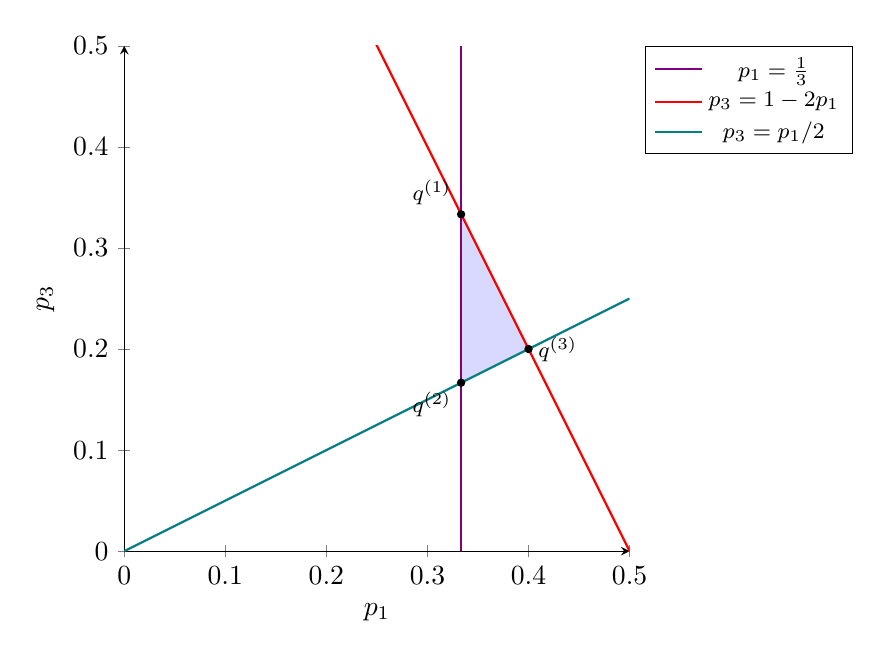
\begin{tikzpicture}
\begin{axis}[
    width=8cm, height=8cm,
    xlabel={$p_1$}, ylabel={$p_3$},
    xmin=0, xmax=0.5,
    ymin=0, ymax=0.5,
    axis lines=left,
    legend pos=outer north east,
    legend style={font=\footnotesize},
    domain=0:0.5,
    samples=2,
]
    \addplot[fill=blue!15, draw=none, forget plot] coordinates {
        (0.3333,0.3333) (0.4,0.2) (0.3333,0.1667)
    } -- cycle;

    \addplot[thick, violet] coordinates {(0.3333,0) (0.3333,0.5)};
    \addlegendentry{$p_1=\tfrac13$}

    \addplot[thick, red] {1-2*x};
    \addlegendentry{$p_3=1-2p_1$}

    \addplot[thick, teal] {x/2};
    \addlegendentry{$p_3=p_1/2$}

    \filldraw (axis cs:0.3333,0.3333) circle (1.3pt) node[above left]{\footnotesize $q^{(1)}$};
    \filldraw (axis cs:0.3333,0.1667) circle (1.3pt) node[below left]{\footnotesize $q^{(2)}$};
    \filldraw (axis cs:0.4,0.2) circle (1.3pt) node[right]{\footnotesize $q^{(3)}$};
\end{axis}
\end{tikzpicture}
\end{center}

The above area shows the possible $p_1, p_3$ pair (which uniquely determines $p_2, p_4$ from the conditions). \\
Therefore, from linearity we get \\
\begin{align*}
    q_1 = (\frac{1}{3}, \frac{1}{3}, \frac{1}{3}, 0) \\
    q_2 = (\frac{1}{3}, \frac{1}{6}, \frac{1}{6}, \frac{1}{6}) \\
    q_3 = (\frac{2}{5}, \frac{1}{5}, \frac{1}{5}, \frac{1}{5})
\end{align*}

\end{sol}
\bigskip

\begin{prob}{5.24}
    Write a short essay discussing how to play the game of \textbf{twenty questions} optimally. [In twenty questions, one player thinks of an object, and the other player has to guess the object using as few binary questions as possible, preferably fewer than twenty.]
\end{prob}
\begin{sol}
    To maximise information obtained, we want to bring the estimated probability of yes/no to be close to 50\% as possible.
    This is impractical to do accurately (since considering all possible objects and its likelihood as the answer are impractical),
    but we can do an approximation by randomly coming up with several objects and think of a question that divides them in 2 (Monte-Carlo approximation, assuming you and the opponent has similar answer distribution).
\end{sol}
\bigskip

\begin{prob}{5.25}
    Show that, if each probability $p_i$ is equal to an integer power of 2 then there exists a source code whose expected length equals the entropy.
\end{prob}
\begin{sol}
    Set the length for symbol with $p_i$ to be $\log\frac{1}{p_i}$ which is an integer. Then,
    $$L(C, X) = \sum_i p_i l_i = \sum_i p_i \log\frac{1}{p_i} = H(X) $$
\end{sol}
\bigskip

\begin{prob}{5.26}
    Make ensembles for which the difference between the entropy and the expected length of the Huffman code is as big as possible.
\end{prob}
\begin{sol}
    We want to maximise $L(C, X) - H(X) = \sum p_i (l_i - \log\frac{1}{p_i})$. \\
    $l_i - \log\frac{1}{p_i} < 1$ so most contribution will come from the symbol that has large $p_i$. We want to make $l_i - \log\frac{1}{p_i}$ as close to 1 for such symbols. \\
    Consider two-symbol ensemble with probabilities $\epsilon$ and $1-\epsilon$ $(0 < \epsilon < 1)$. Then, $L(C, X) = 1$ regardless of the value of $\epsilon$. \\
    However, $H(X) = H_2(\epsilon) \rightarrow 0$ as $\epsilon \rightarrow 0$. \\
    Hence the ensemble with an extremely skewed probability has a difference between the entropy $\approxeq$ 1, which is as big as it gets. 
\end{sol}

\begin{prob}{5.27}
    A source $X$ has an alphabet of eleven characters
\[
\{\mathbf{a}, \mathbf{b}, \mathbf{c}, \mathbf{d}, \mathbf{e}, \mathbf{f}, \mathbf{g}, \mathbf{h}, \mathbf{i}, \mathbf{j}, \mathbf{k}\},
\]
all of which have equal probability, $1/11$.

\noindent Find an optimal uniquely decodeable symbol code for this source. How much greater is the expected length of this optimal code than the entropy of $X$?
\end{prob}
\begin{sol}
With Huffman coding, \\
\begin{tabular}{ c c c }
    symbol & codeword & length \\
    a & 000 & 3 \\
    b & 001 & 3 \\
    c & 010 & 3 \\
    d & 011 & 3 \\
    e & 1000 & 4 \\
    f & 1001 & 4 \\
    g & 1010 & 4 \\
    h & 1011 & 4 \\
    i & 1100 & 4 \\
    j & 1101 & 4 \\
    k & 111 & 3
\end{tabular}\\

$$H(X) = \log_2 11 = 3.459$$
$$L(C, X) = \frac{3 \times 5 + 4 \times 6}{11} = 3.545$$
$$L(C, X) - H(X) = 0.08645$$
\end{sol}
\bigskip

\begin{prob}{5.28}
Consider the optimal symbol code for an ensemble $X$ with alphabet size $I$ from which all symbols have identical probability $p = 1/I$. $I$ is not a power of 2.

\noindent Show that the fraction $f^+$ of the $I$ symbols that are assigned codelengths equal to
\begin{equation}
l^+ \equiv \lceil \log_2 I \rceil
\end{equation}
satisfies
\begin{equation}
f^+ = 2 - \frac{2^{l^+}}{I}
\end{equation}
and that the expected length of the optimal symbol code is
\begin{equation}
L = l^+ - 1 + f^+.
\end{equation}
By differentiating the excess length $\Delta L \equiv L - H(X)$ with respect to $I$, show that the excess length is bounded by
\begin{equation}
\Delta L \le 1 - \frac{\ln(\ln 2)}{\ln 2} - \frac{1}{\ln 2} = 0.086.
\end{equation}
\end{prob}
\begin{sol}
When all symbols have equal probability, the merging process will be the same as if there are $2^{\lceil \log_2 I \rceil}$ symbols (a full tournament) but with $2^{l+} - I$ dummies and the dummies being merged with their adjacents.
The way the symbols are allocated to the tournament slots is from the left slots of the lowest stage, left to right (will fill in all) and then right slots (, left to right). \\
Then, $2^{l+} - I$ symbols will not have their neighbour so will have length $l^+ - 1$ while the remaining will have length $l^+$. Hence, 
\begin{align*}
    I(1 - f^+) &= 2^{l+} - I \\
    If^+ &= 2I - 2^{l+} \\
    f^+ &= 2 - \frac{2^{l+}}{I}
\end{align*}

Also, 
\begin{align*}
    L &= l^+ f^+ + (l^+ - 1)(1 - f^+) \\
    &= l^+ f^+ + l^+ - l^+ f^+ - 1 + f^+ \\
    &= l^+ - 1 + f^+
\end{align*}

Now, 
\begin{align*}
    \Delta L &\equiv L - H(X) \\
    &= \lceil \log_2 I \rceil - 1 + 2 - \frac{2^{l+}}{I} - \log_2 I\\
    &= 1 - \frac{2^{l+}}{I} + \lceil \log_2 I \rceil - \log_2 I \\
    \frac{d\Delta L}{dI} &= \frac{2^{l+}}{I^2} + 0 - \frac{1}{I \ln 2} \quad (\because I \text{ not power of 2})\\
\end{align*}
\begin{align*}
    &\frac{d\Delta L}{dI} = 0 \\
    \iff&2^{l+} - \frac{I}{\ln 2} = 0 \\
    \iff&I = 2^{l+}\ln 2
\end{align*}
To confirm this critical point is a maximum, consider the second derivative:
\begin{align*}
    \frac{d^2 \Delta L}{dI^2} = -\frac{2 \cdot 2^{l+}}{I^3} + \frac{1}{I^2 \ln 2}
\end{align*}
Evaluating at $I = 2^{l+}\ln 2$,
\begin{align*}
    \frac{d^2 \Delta L}{dI^2}\bigg|_{I = 2^{l+}\ln 2} &= \frac{1}{I^2}\left(\frac{1}{\ln 2} - \frac{2 \cdot 2^{l+}}{I}\right) \\
    &= \frac{1}{I^2}\left(\frac{1}{\ln 2} - \frac{2 \cdot 2^{l+}}{2^{l+}\ln 2}\right) \\
    &= \frac{1}{I^2}\left(\frac{1}{\ln 2} - \frac{2}{\ln 2}\right) = -\frac{1}{I^2 \ln 2} < 0,
\end{align*}
so $\Delta L$ is concave at this point, confirming it is a (local, and since it is the only critical point, global) maximum on the interval. So
\begin{align*}
    \Delta L &\leq 1 - \frac{1}{\ln 2} + \log_2 \frac{2^{l+}}{I} \\
    &= 1 - \frac{1}{\ln 2} - \log_2(\ln 2) \\
    &= 1 - \frac{\ln(\ln 2)}{\ln 2} - \frac{1}{\ln 2} \\
    &= 0.086
\end{align*}

\end{sol}
\bigskip

\begin{prob}{5.29}
    Consider a sparse binary source with $\mathcal{P}_X = \{0.99, 0.01\}$. Discuss how Huffman codes could be used to compress this source \textit{efficiently}. Estimate how many codewords your proposed solutions require.
\end{prob}
\begin{sol}
Let a be the symbol that has probability 0.99 and b 0.01. Then if we pair two symbols and apply Huffman coding, \\

\begin{tabular}{c c c}
    string & probability & codeword \\
    \hline
    aa & $0.9801$ & 0 \\
    ab & $0.0099$ & 10 \\
    ba & $0.0099$ & 110 \\
    bb & $0.0001$ & 111 \\
\end{tabular}\\

Expected length $= 1 \times 0.9801 + 2 \times 0.0099 + 3 \times 0.0099 + 3 \times 0.0001 = 1.0299$. \\
Then, Expected length per source symbol $= 0.51495$ which is much less than pure 1 symbol encoding. \\
The drawback, however, is that odd length source code cannot be encoded.
\end{sol}
\bigskip


\bigskip

% template
\begin{prob}{}
\end{prob}
\begin{sol}
\end{sol}
\bigskip


\end{document}



